\chapter{Implementasi dan Pengujian Perangkat Lunak}
\label{chap: Implementasi dan Pengujian Perangkat Lunak}

Bab ini terdiri atas tiga bagian, yaitu Implementasi Data JSON, Implementasi Perangkat Lunak dan Pengujian Perangkat Lunak. Bagian implementasi data JSON akan berisi hasil implementasi perangkat lunak dan pengujian fungsional yang telah dilakukan.

\section{Implementasi Data JSON}
\label{sec: Implementasi Data JSON}

Dalam pembangunan pohon kurikulum digunakan JSON sebagai data pembuat grafik. JSON dibangkitkan dengan cara diubah menjadi \textit{dot}. Hasilnya berupa grafik yang berbentuk pohon kurikulum. JSON selanjutnya diunggah dan diakses melalui \textit{url} \url{https://github.com/ftisunpar/data} dan dapat dilihat pada bagian prasyarat. 

\section{Implementasi Perangkat Lunak}
\label{sec: Implementasi Perangkat Lunak}

Pada bagian ini akan dibahas mengenai implementasi perangkat lunak yang telah dibangun. Sub bab ini terdiri atas dua bagian, yaitu hasil implementasi perangkat lunak dan Pengujian fungsional.

\subsection{Hasil Implementasi}
\label{sec: Hasil Implementasi}

Kode program pada perangkat lunak ditulis dalam bahasa pemrograman \textit{javascript} dengan cara membangkitkan dari JSON ke \textit{DOT}. Hasil implementasi berupa pohon kurikulum yang visualisasinya menggunakan \textit{viz.js} dan sudah memakai \textit{engine DOT}. Perangkat lunak dapat dilihat seperti gambar di bawah ini.

\begin{figure}[H]
		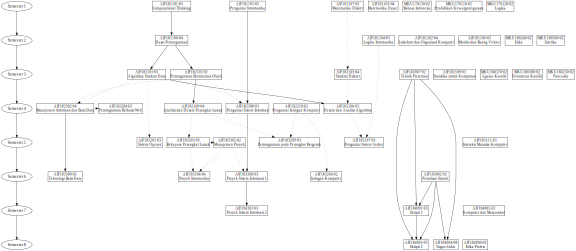
\includegraphics[scale = 0.7]{dot.png}
		\caption{Hasil Implementasi}
		\label{fig: pohon kurikulum}
\end{figure}	 

Pada gambar \ref{fig: pohon kurikulum} terlihat setiap semester memiliki mata kuliah yang berisi semester, kode mata kuliah, jumlah sks, dan nama mata kuliah. Lalu mata kuliah yang memiliki prasyarat akan ditunjuk oleh panah. Syarat yang menjadi patokan adalah syarat tempuh, syarat lulus, atau pengambilan secara bersamaan.

\section{Pengujian Perangkat Lunak}
\label{sec: Pengujian Perangkat Lunak}

Pada bab ini akan dibahas mengenai pengujian perangkat lunak yang dibangun. Pengujian yang dilakukan adalah pengujian fungsional dan pengujian eksperimental. Pengujian fungsional bertujuan untuk memastikan bahwa seluruh fungsi perangkat lunak yang dibangun berjalan sesuai dengan rencana dan pengujian eksperimental bertujuan untuk mengetahui apa saja \textit{engine} yang dapat dipakai dalam membangun perangkat lunak.

\subsection{Pengujian Fungsional}
\label{sec: Pengujian Fungsional}
Dalam sub bab ini akan dilakukan pengujian fungsional untuk mengetahui fungsi-fungsi yang terdapat
pada perangkat lunak dapat berjalan sesuai dengan yang diharapkan. Status pengujian dibagi
menjadi dua yaitu "ok" dan "gagal". Di bawah ini Pengujian fungsi pohon kurikulum:

\begin{table}[H]
\begin{center}
\caption{Hasil Pengujian Fungsional}
\begin{tabular}{{|p{2cm}|p{3cm}|p{4cm}|p{1cm}|}}
\hline
  Pengujian & Tujuan Pengujian & Hasil Pengujian & Status \\
\hline
  Memanggil fungsi rankSep & Mengeluarkan node semester dan kode mata kuliah wajib & node semester satu sampai delapan dan kode mata kuliah berhasil diketahui & ok\\ \hline
	Memanggil fungsi nodesMatkul & fungsi nodesMatkul akan mengeluarkan label yang berisi kode, sks, dan nama mata kuliah & kode, sks, dan nama mata kuliah wajib berhasil ditampilkan & ok\\ \hline
	Memanggil fungsi edgesMatkul & Mata kuliah yang mempunyai prasyarat bisa diketahui melalui petunjuk arah & Mata kuliah yang memiliki prasyarat akan ditunjuk sesuai prasyarat. Jika syaratnya lulus maka garis akan lurus jika syaratnya tempuh garis putus-putus & ok\\ \hline
   
\end{tabular}
\end{center}
\end{table}
